\section{Реализация платформы для интерактивного формирования запросов к языковым и генеративным нейросетям}

В данном разделе подробно описывается реализация программной платформы, предназначенной для интерактивного формирования запросов к современным языковым моделям и генеративным нейросетям. Целью разработки было создать удобный и гибкий инструмент, позволяющий пользователям составлять сложные запросы к моделям искусственного интеллекта (как текстовым, так и визуальным), используя наглядный интерфейс. Такой подход упрощает работу с крупными языковыми и генеративными моделями, скрывая сложность формулировки текстовых запросов \cite{lakera:2025} и последовательной обработки данных.

Разрабатываемая платформа реализована как клиент--сервер: \textbf{frontend} (клиентское веб-приложение) создан на основе Vue 3 с использованием хранилища состояний Pinia, а серверная часть реализована на фреймворке FastAPI на языке Python\cite{fastapi:practicum}. В качестве базы данных используется PostgreSQL с подключённым расширением pgvector для хранения и поиска векторных представлений данных. Данный стек технологий был выбран с учётом требований к интерактивности интерфейса, необходимости вызывать внешние API генеративных моделей, а также для обеспечения возможности масштабирования и расширения функциональности.

Ниже приводится структурированное описание архитектуры системы и ключевых компонентов реализации. Сначала рассматривается общая архитектура платформы и взаимодействие между её компонентами. Затем описывается клиентская часть, в том числе реализация drag-and-drop интерфейса для формирования запросов. После этого подробно изложена работа серверной части: обработка запросов, интеграция с внешними API (для генерации текстов и изображений) и использование векторного поиска для улучшения качества результатов. Завершает раздел \textbf{вывод} с описанием достигнутых результатов разработки и перспектив расширения системы.

\subsection{Архитектура платформы}
\begin{figure}[htbp]
    \centering
    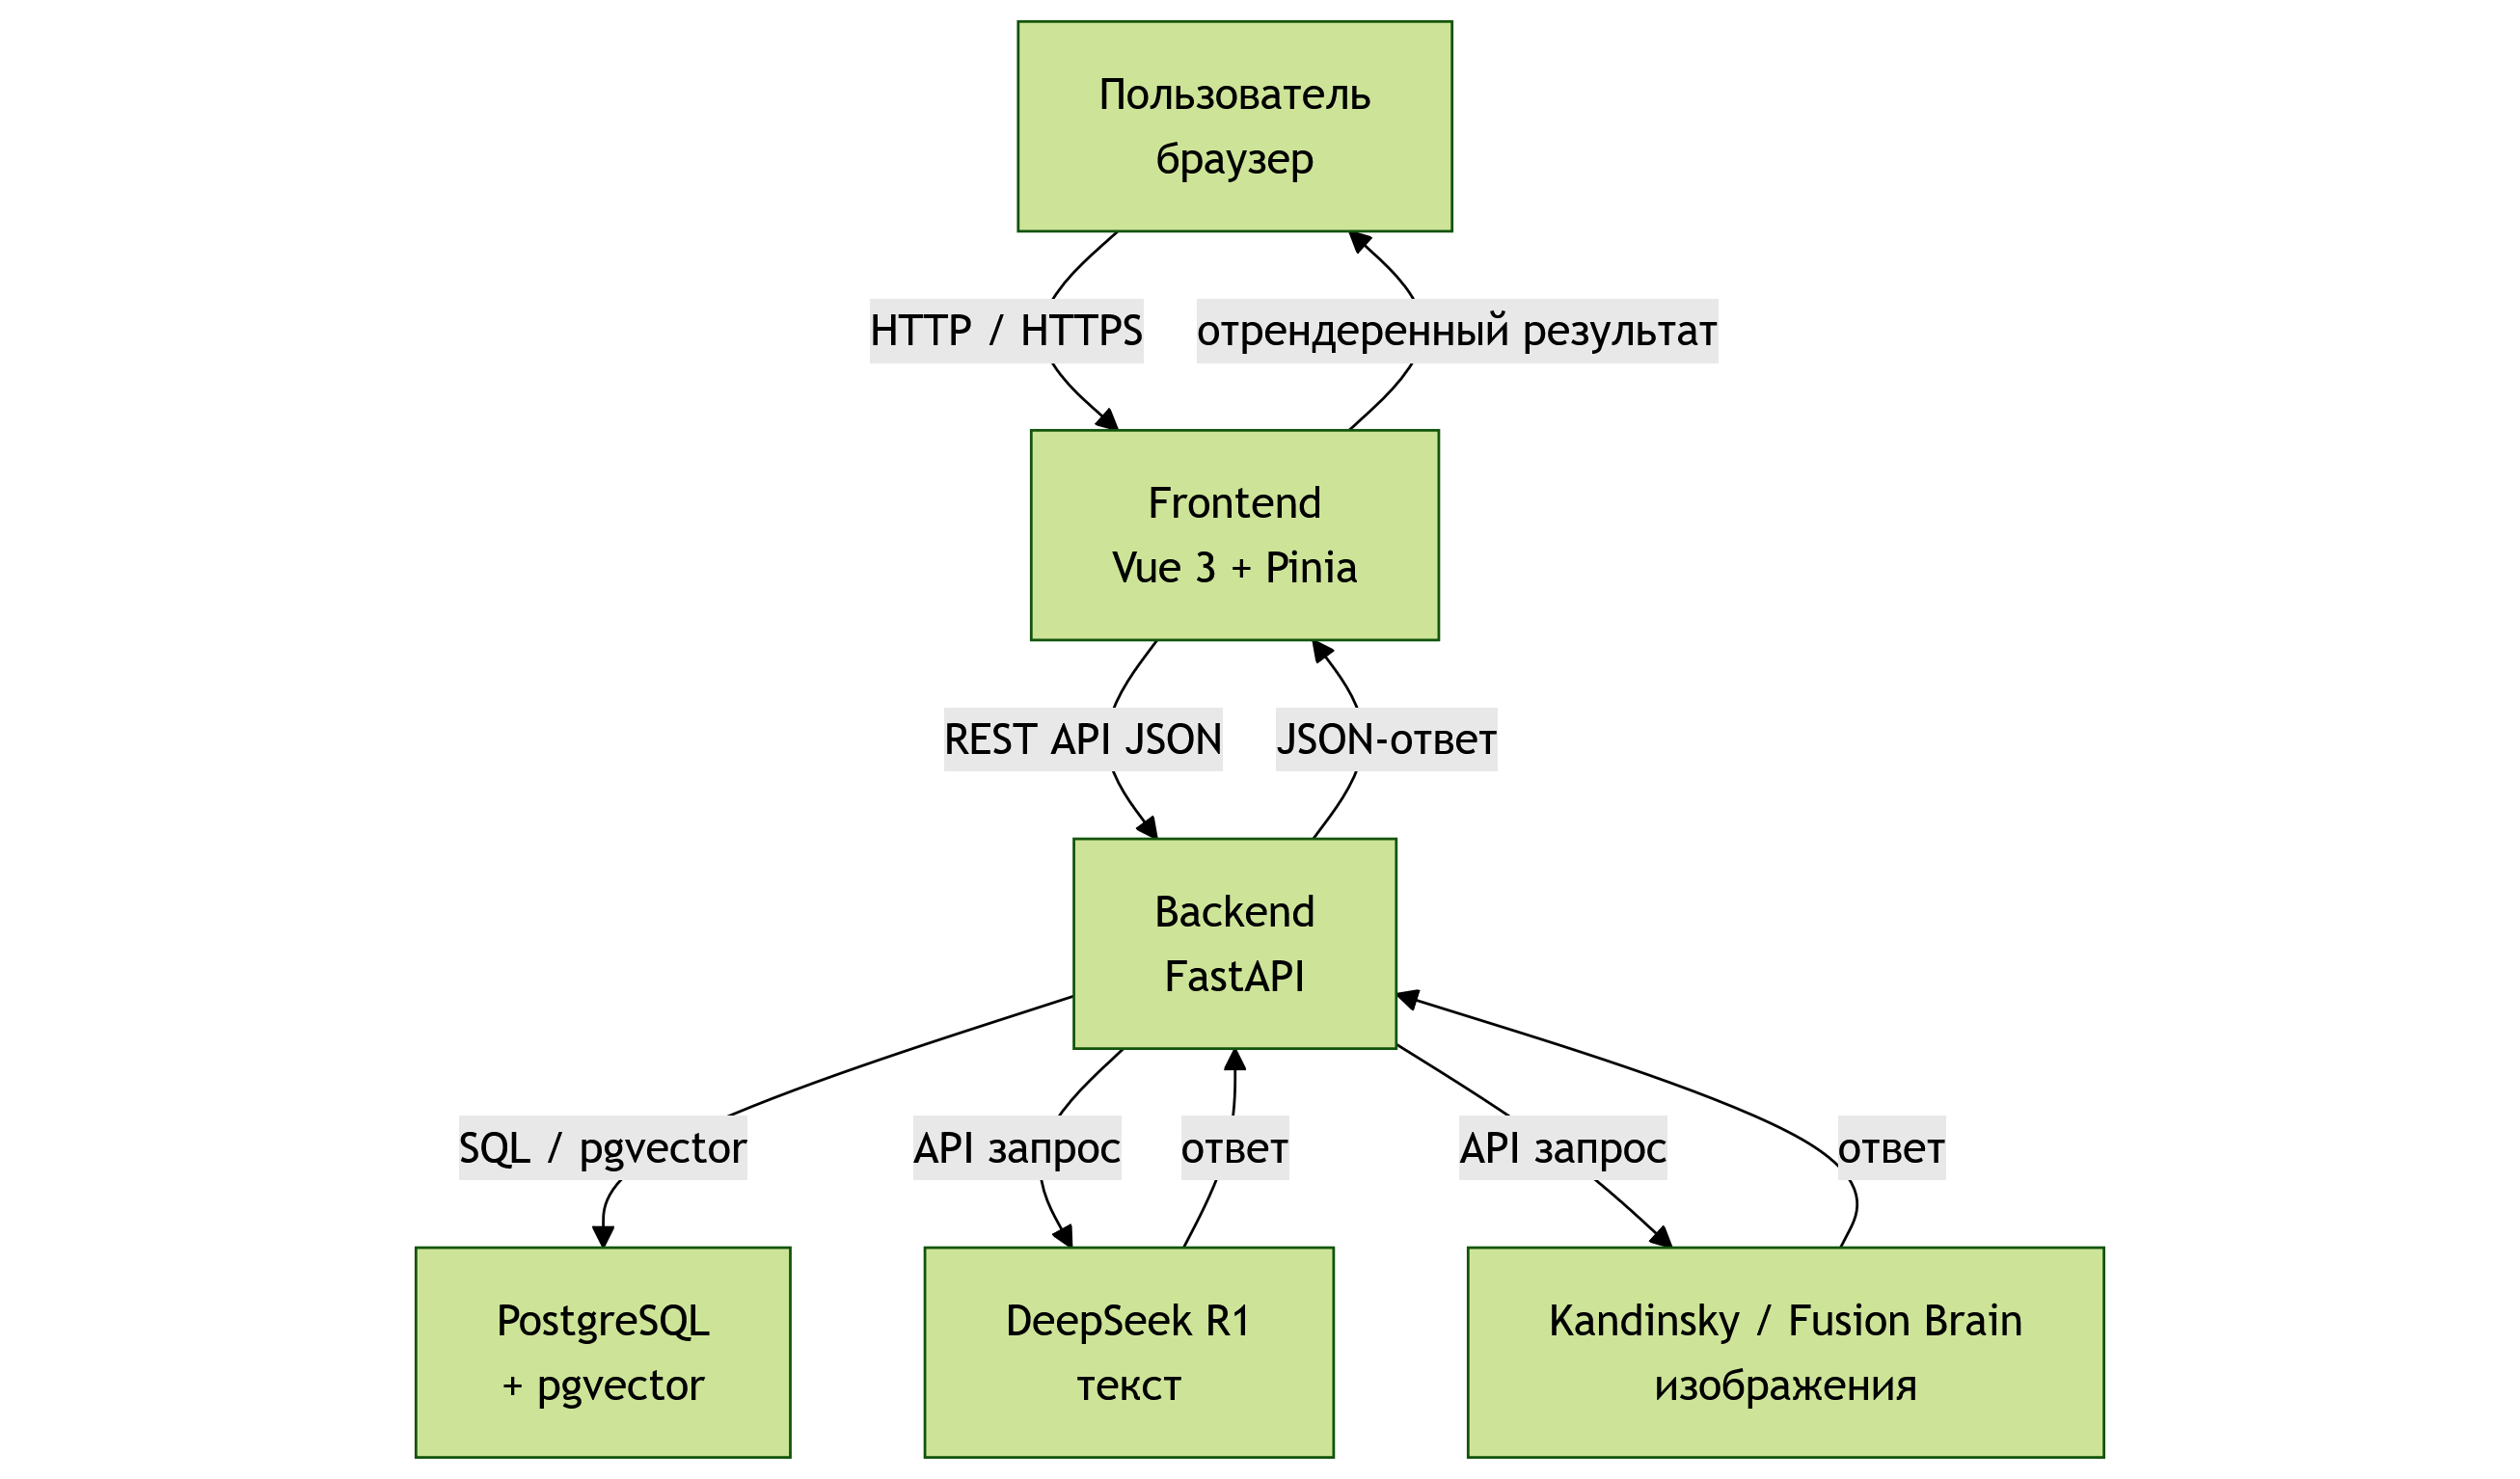
\includegraphics[width=0.8\textwidth]{picture/app-architecture.png}
    \caption{Архитектура платформы}\label{architecture}
\end{figure}
 Платформа имеет распределённую архитектуру типа «клиент–сервер». Это означает, что функциональность разделена между клиентским приложением, выполняющимся в браузере пользователя и сервером. На рисунке \ref{architecture} представлена структурная схема архитектуры системы с основными компонентами и потоками данных.

Как показано на схеме, центральным звеном является веб-сервер API, реализованный на FastAPI. Этот сервер принимает входящие запросы от клиентского приложения по протоколу HTTP(S) и отвечает на них. Взаимодействие клиента и сервера происходит по REST API: для каждой функции предусмотрен соответствующий эндпойнт. Например, могут быть маршруты \verb|complete prompt| (для дополнения детализации), \verb|valuate prompt| (для оценки), \verb|transform prompt| (для реструктуризации) и \verb|preview| (для получения результата генерации). Клиентское приложение обращается к этим конечным точкам, передавая необходимые данные (тексты промптов, параметры) в формате JSON, и получает от сервера ответы, также закодированные в JSON (кроме случаев, когда передаются двоичные данные изображения). Обмен происходит по сети, предпочтительно с использованием шифрования (HTTPS) для безопасности.

Клиентская часть (Vue.js SPA) – это одностраничное приложение, загружаемое в браузер. Оно отвечает за отображение UI и интерактивность. После загрузки (HTML, CSS, JS) клиент устанавливает связь с сервером через AJAX-запросы (например, с помощью fetch API или библиотеки axios) к REST API. Вся логика по обновлению интерфейса – на стороне клиента: перемещение токенов, обновление текста, визуализация оценки (например, индикатор качества) – выполняется средствами JavaScript внутри браузера. Vue.js, являясь реактивным фреймворком, упрощает реализацию динамических компонентов интерфейса\cite{vuejs:wiki}. Например, текстовое поле и список токенов могут быть связанными реактивными данными: изменение одного автоматически отражается в другом. Клиент также обрабатывает элементы управления – кнопка «Оценить» может просто вызывать соответствующую функцию JS, которая отправит запрос на сервер и по получении ответа обновит отображаемую оценку. Аналогично, нажатие «Preview» инициирует последовательность: показать индикатор загрузки, отправить промпт на сервер, дождаться ответа и затем либо отобразить сгенерированный текст, либо встроить полученное изображение (например, через создание HTML-элемента \<img\> с полученными данными). Таким образом, клиент выполняет роль презентационного слоя, обеспечивая удобство для пользователя и минимизируя задержки взаимодействия (многие операции, не требующие ресурсов сервера, происходят мгновенно за счёт реактивности Vue).

Серверная часть (FastAPI) – сердце бизнес-логики платформы. FastAPI выбран благодаря его современной архитектуре, оптимизированной под высоконагруженные API и удобство разработки. Приложение FastAPI запускается, как правило под управлением ASGI--сервера (например, Uvicorn), способного обрабатывать асинхронные запросы. Основные компоненты на стороне сервера:
\begin{enumerate}[label=\arabic*]
    \item Контроллеры (роуты) API. В FastAPI разработаны обработчики для каждого метода API. Они принимают входные данные (автоматически распарсенные из JSON благодаря Pydantic-моделям), выполняют требуемые действия (например, вызывают модель или делают запрос к БД) и формируют ответ. Каждый такой контроллер работает по принципу: получить запрос -> вызвать соответствующую внутреннюю функцию или метод -> вернуть результат пользователю. Например, контроллер \verb|evaluate prompt| получив JSON с полем \verb|prompt|: "текст запроса", передаст эту строку в модуль оценки качества и вернёт клиенту JSON с полем score: 78 (пример).
    \item Модуль интеграции с DeepSeek. Поскольку модель DeepSeek используется через API Серверное приложение должно обращаться к модели DeepSeek через её REST-API и хранить необходимые параметры подключения (ключ доступа, базовый URL) в памяти, а также предоставлять методы для генерации текста. При запуске сервера выполняется инициализация клиента API: создаётся singleton-объект DeepSeekClient, который содержит токен, настройки таймаутов и общие параметры (например, модель = deepseek-llm-67b-chat). Такой подход тоже считается встроенным (embedded), но модель «встроена» логически — она доступна сервису как удалённый ресурс, а не как локальный файл весов\cite{deepseek:docs}.Взаимодействие с DeepSeek осуществляется через HTTP-вызовы: сервер формирует JSON-запрос на основе пользовательского промпта (поля model, messages, temperature и т. д.), отправляет его методом POST на эндпоинт /v1/chat/completions и получает ответ с сгенерированным текстом. Далее текст при необходимости фильтруется или обрезается до заданной длины и возвращается клиенту. Благодаря статическому объекту DeepSeekClient соединение можно переиспользовать, что снижает сетевые накладные расходы и ускоряет получение ответов по сравнению с созданием нового соединения для каждой генерации.
    \item Модуль интеграции с Fusion Brain API. В случаях, когда требуется сгенерировать изображение, сервер выполняет роль клиента к внешнему API. Он делает HTTP-запрос (например, POST) к службе Fusion Brain, включая в него текст промпта и необходимые параметры (версия модели, желаемое разрешение изображения и т.д.). В ответ Fusion Brain возвращает данные изображения. Согласно документации, Kandinsky 3.1 позволяет получать изображения размером до 1024×1024; для предпросмотра сервер может запрашивать, к примеру, изображение 512×512 пикселей, чтобы сократить время ответа\cite{fusionbrain:docs}. Полученное изображение может приходить закодированным (например, URL ссылки на изображение или бинарные данные). Сервер, получив результат, преобразует его в формат, пригодный для пересылки клиенту. Наиболее прямолинейный способ – переслать изображение как набор байт (в base64) или как ссылку, проксируемую через сервер. В реализации платформы может использоваться проксирование: сервер сохраняет картинку во временном хранилище (или просто держит в памяти) и отдаёт фронту по тому же API (например, ответ на preview для изображения содержит URL вида media preview123.png или непосредственный Base64). Клиентская часть затем отображает картинку пользователю. Взаимодействие с внешним API должно быть безопасным: ключ API Fusion Brain хранится на сервере (в конфигурации), и ни при каком условии не отправляется на клиент. Запросы должны выполняться асинхронно, чтобы не блокировать другие процессы сервера.
    \item Модуль работы с базой данных. Серверное приложение взаимодействует с PostgreSQL для хранения постоянных данных. Это включает регистрацию/авторизацию пользователей и сохранение истории запросов. История запросов может храниться в виде таблицы: пользователь, текст промпта, время, возможно оценка и предпросмотр (например, ссылка на сохранённый результат). Обращения к базе данных реализованы через ORM (например, SQLAlchemy) либо через драйвер asyncpg для асинхронной работы. Использование ORM обеспечивает защиту от SQL-инъекций и удобство разработки – запросы к базе генерируются автоматически, что повышает надёжность хранения данных\cite{postgresql:skillfactory}, \cite{postgresql:wiki}. PostgreSQL, будучи одной из наиболее развитых свободных СУБД, гарантирует целостность данных и поддерживает все необходимые функции (ACID-транзакции, индексацию и пр.), что важно для ведения истории запросов без потерь. 
\end{enumerate}
Архитектура поддерживает масштабирование: при возросшей нагрузке клиентская часть приложения может быть вынесена на отдельный CDN, а серверная часть – развёрнута в виде нескольких экземпляров за балансировщиком нагрузки. База данных может быть отдельно вынесена на кластер PostgreSQL для обеспечения высокой доступности. Так как сервер Stateless (не хранит сессии в памяти, вся важная информация – в БД), то масштабировать его горизонтально несложно. В расчёте на целевое применение (ограниченное число пользователей) текущая архитектура (один бекенд-инстанс с моделью) считается достаточной и оптимальной по простоте.

Взаимодействие компонентов происходит по следующему сценарию. Пользователь посредством клиента формирует запрос (например, текстовое описание задачи или сцены для генерации изображения). При отправке запроса клиентское приложение собирает все необходимые данные (включая текстовые поля, выбранные опции, прикреплённые изображения или другие элементы) и отправляет их на сервер через HTTP-запрос к API. Серверная часть принимает запрос, анализирует его тип и содержимое: если требуется текстовая генерация, вызывается соответствующий метод, если генерация изображения — другой метод. Перед обращением к модели сервер может обратиться к базе знаний: например, выполнить векторный поиск по базе ранее сохранённых данных для нахождения дополнительного контекста (релевантных текстов) и объединить их с запросом пользователя. Затем сервер формирует запрос к внешнему API нужной модели (с учётом ключа доступа и формата, требуемого API), и ожидает ответа. Получив результат от модели (сгенерированный текст или изображение), сервер производит сохранение результата в базу (при необходимости) и возвращает результат клиенту. Фронтенд, получив ответ, отображает пользователю сгенерированный контент. В случае изображения оно выводится прямо на страницу, в случае текста — отображается в виде ответа ассистента. При этом интерфейс может позволять пользователю далее уточнять запрос (например, задать уточняющий вопрос или отредактировать сгенерированный результат и отправить повторно), образуя интерактивный цикл работы.

Подобная архитектура обеспечивает гибкость: компоненты чётко разделены, что даёт возможность модифицировать их независимо. Например, можно заменить модель генерации текста на другую, не затрагивая интерфейс, достаточно изменить вызов в серверной части. Или можно развивать клиентскую часть приложения (добавлять новые элементы взаимодействия) без изменения логики генерации на сервере. Использование стандартных веб-технологий (HTTP API, JSON) для обмена данными между клиентом и сервером обеспечивает совместимость и простоту отладки.

\subsection{Интерфейс платформы}

Клиентская часть платформы реализована как одностраничное приложение на Vue 3, что позволяет создать динамичный интерфейс, обновляющийся без полной перезагрузки страницы. Одной из ключевых задач клиента было обеспечить \textit{drag-and-drop} интерфейс для интерактивного составления запросов. Это означает, что пользователю предоставляется возможность добавлять, удалять и менять местами различные блоки запроса с помощью мыши, просто перетаскивая элементы на экране.

Для реализации drag-and-drop функциональности были использованы возможности HTML5 Drag and Drop API и компоненты Vue. В частности, элементы интерфейса, представляющие части запроса (например, фрагмент текста инструкции, блок для ввода вопроса, изображение-пример или параметры генерации), сделали перетаскиваемыми с помощью атрибутов \verb|draggable| и соответствующих обработчиков событий (\verb|dragstart|, \verb|dragover|, \verb|drop| и т.д.). Когда пользователь начинает перетаскивание элемента, приложение запоминает (через Pinia-хранилище) текущий переносимый объект. Когда происходит сброс (drop) элемента на новую позицию или область, обновляется состояние списка блоков запроса. Pinia отвечает за централизованное хранение структуры запроса: каждый блок может быть представлен объектом с полями, описывающими его тип (текст, изображение, параметр), содержимое (например, сам текст или ссылка на файл изображения) и, возможно, дополнительные настройки.

Благодаря реактивности Vue, обновление состояния Pinia автоматически приводит к перерисовке списка блоков на экране в новом порядке. Это даёт плавный пользовательский опыт при сборке запроса из блоков. Пользователь может, к примеру, перетащить в область запроса готовый шаблон подсказки\cite{copilotworks:promptgen} из библиотеки слева, затем добавить свои уточнения текстом, а затем перетянуть специальный блок, обозначающий место, куда будет подставлен результат другого запроса. Такой механизм особенно полезен для составления сложных запросов, например, когда требуется сгенерировать текст по определённому шаблону или выполнить несколько шагов генерации (сначала текст, потом на основе этого текста — изображение).

Стоит отметить, что Pinia значительно упростила реализацию управления состоянием по сравнению с классическим Vuex (Vue 2), благодаря более простому синтаксису и TypeScript-совместимости. Были созданы отдельные store (хранилища) Pinia для разных частей состояния приложения. Например, один store хранит текущий состав блоков запроса (их список и свойства), другой — историю предыдущих запросов и ответов, третий — настройки пользователя (выбранные модели генерации, параметры вроде температуры генерации текста, желаемого разрешения изображения и т.п.). Разделение на несколько хранилищ повышает модульность: логика по управлению историей отделена от логики формирования текущего запроса.

Ниже приведён упрощённый пример компонента Vue, реализующего область с перетаскиваемыми блоками запроса. В этом фрагменте кода показано, как можно выводить список блоков и обеспечивать их перетаскивание с помощью директивы \verb|v-for| и событий drag-and-drop:
\newpage
\begin{lstlisting}[language=HTML]
       <div class="query-builder" @drop="onDrop" @dragover.prevent>
             <div class="query-block" v-for="(block, index) in blocks" :key="block.id" draggable="true" @dragstart="onDragStart(block, index)">
               <div v-if="block.type === 'text'"> {{ block.text }} </div> <div v-else-if="block.type === 'image'">
                <img :src="block.preview" alt="Image" /> </div> <div v-else-if="block.type === 'param'">
                 <span>{{ block.name }}: {{ block.value }}</span>
                </div>
                </div>
              </div>
\end{lstlisting}

\vspace{-0.5\baselineskip} 
В приведённом фрагменте шаблона Vue каждый элемент \verb|<div class="query-block">| представляет отдельный блок запроса, который может быть текстовым, изображением или блоком параметров. Атрибут \verb|draggable="true"| делает элемент перетаскиваемым. Обработчик \verb|@dragstart| привязан к методу \verb|onDragStart|, который сохраняет переносимый блок и его индекс. Обработчик \verb|@drop| на контейнере \verb|query-builder| вызывается, когда блок отпущен в новой позиции; внутри метода \verb|onDrop| происходит обновление порядка блоков в списке \verb|blocks|. Использование \verb|@dragover.prevent| необходимо, чтобы разрешить сброс элементов (по умолчанию браузер запрещает сброс для необработанных зон). Таким образом, этот компонент даёт возможность динамически менять состав и последовательность частей запроса.

Другой важной частью клиента является форма ввода и отображения результатов. Над областью сборки запроса размещены поля для ввода основного текста запроса пользователя, а также (опционально) для указания негативных подсказок (\textit{negative prompt} для генерации изображений, чтобы исключить нежелательные детали), выбора модели или пресета настроек. Рядом располагаются кнопки: "Сгенерировать текст", "Сгенерировать изображение" и т.п., в зависимости от выбранного типа задачи. После нажатия соответствующей кнопки собранная структура запроса отправляется на сервер.
\begin{figure}[h]
    \centering
    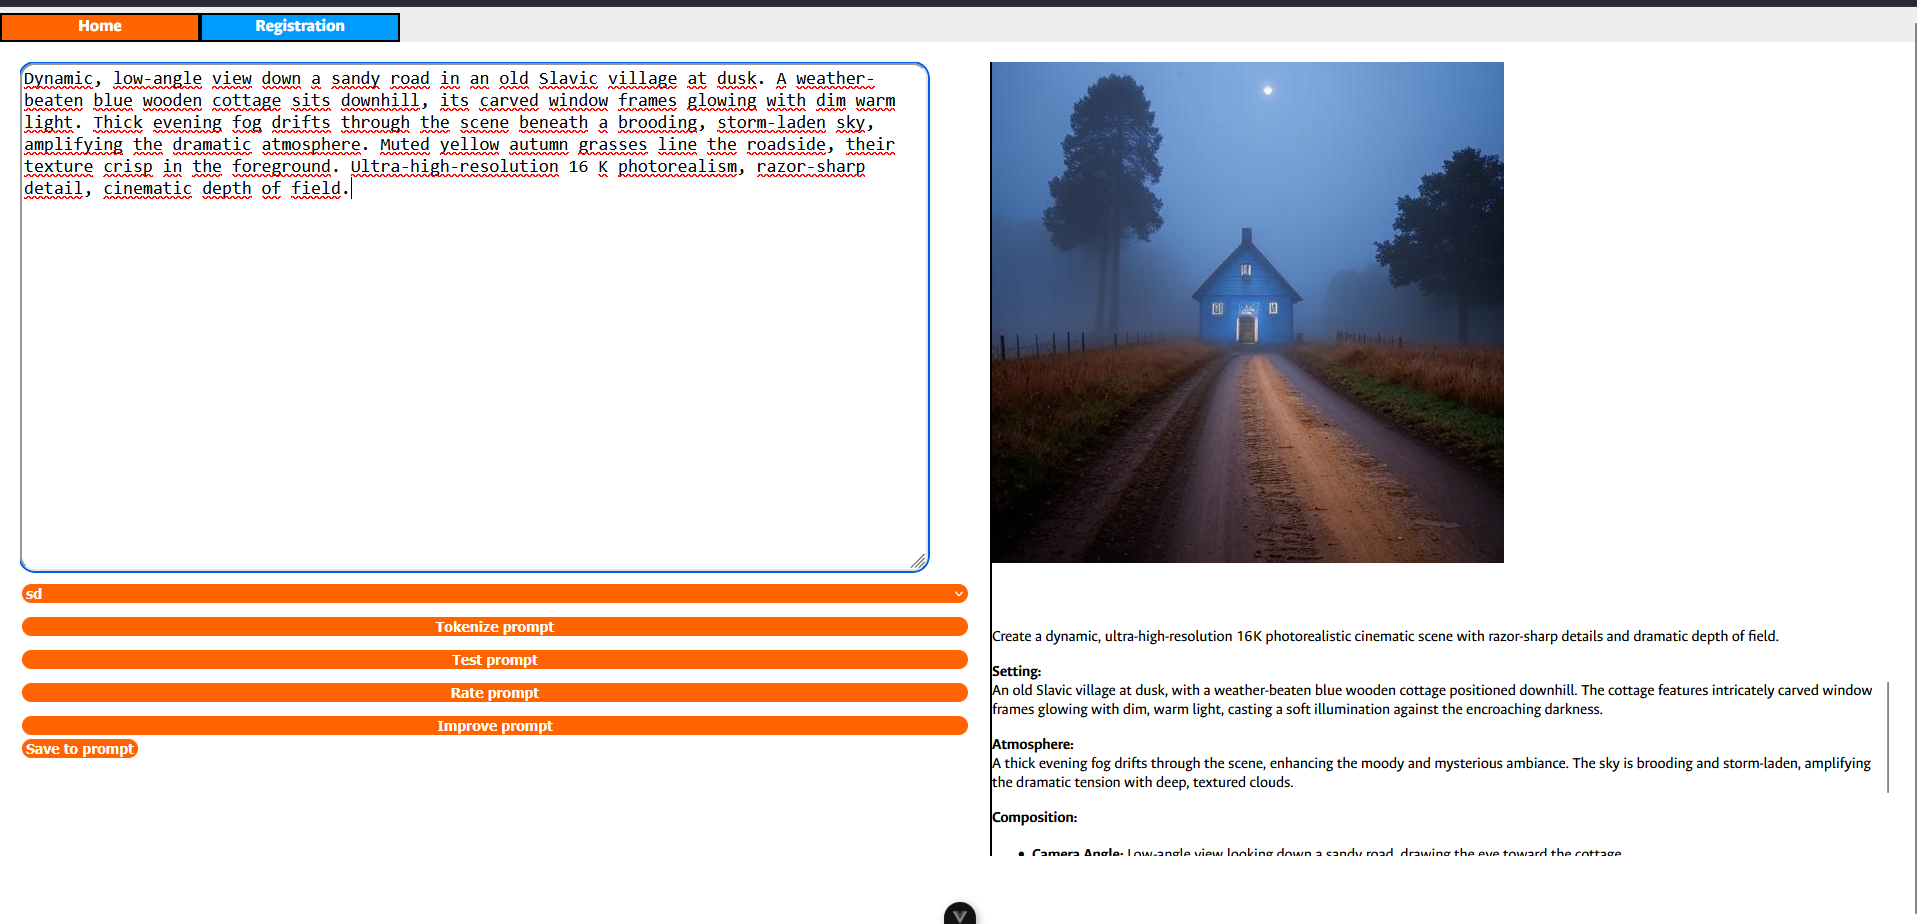
\includegraphics[width=0.8\textwidth]{picture/interface-screenshot_1.png}
    \caption{Скриншот платформы}\label{interface-screenshot}
\end{figure}
Для отображения результатов на странице предусмотрены соответствующие области: текстовые результаты показываются в виде ленты с историей запросов что можно увидеть на рисунке \ref{interface-screenshot}, изображения — в виде изображений в истории запросов. Все эти элементы также управляются состоянием Pinia: результат генерации (например, полученный от модели текст) сохраняется в историю запросов и отображается вместе с исходным запросом.

Таким образом, клиент обеспечивает интерактивное и наглядное взаимодействие: пользователь манипулирует блоками запроса и сразу видит, как формируется итоговый запрос, а после отправки — мгновенно получает отображение результата. Высокая отзывчивость интерфейса достигается благодаря возможностям Vue 3 по оптимизации обновлений DOM и использованию reactive-переменных, а также благодаря разгрузке тяжёлых вычислений на сервер и внешние сервисы.

\subsection{Серверная часть и интеграция с внешними API}

Серверное приложение, реализованное на FastAPI, отвечает за приём запросов от клиента, их обработку и взаимодействие с моделями ИИ через внешние API. FastAPI был выбран по нескольким причинам: во-первых, он обеспечивает высокую производительность и низкую задержку благодаря использованию асинхронного подхода (на базе UVicorn/Starlette); во-вторых, имеет удобный механизм автоматической генерации документации API (OpenAPI/Swagger), что упрощает отладку и тестирование; в-третьих, написан на Python, что облегчает интеграцию с Python-библиотеками для машинного обучения и вызова внешних API.
\begin{figure}[h]
    \centering
    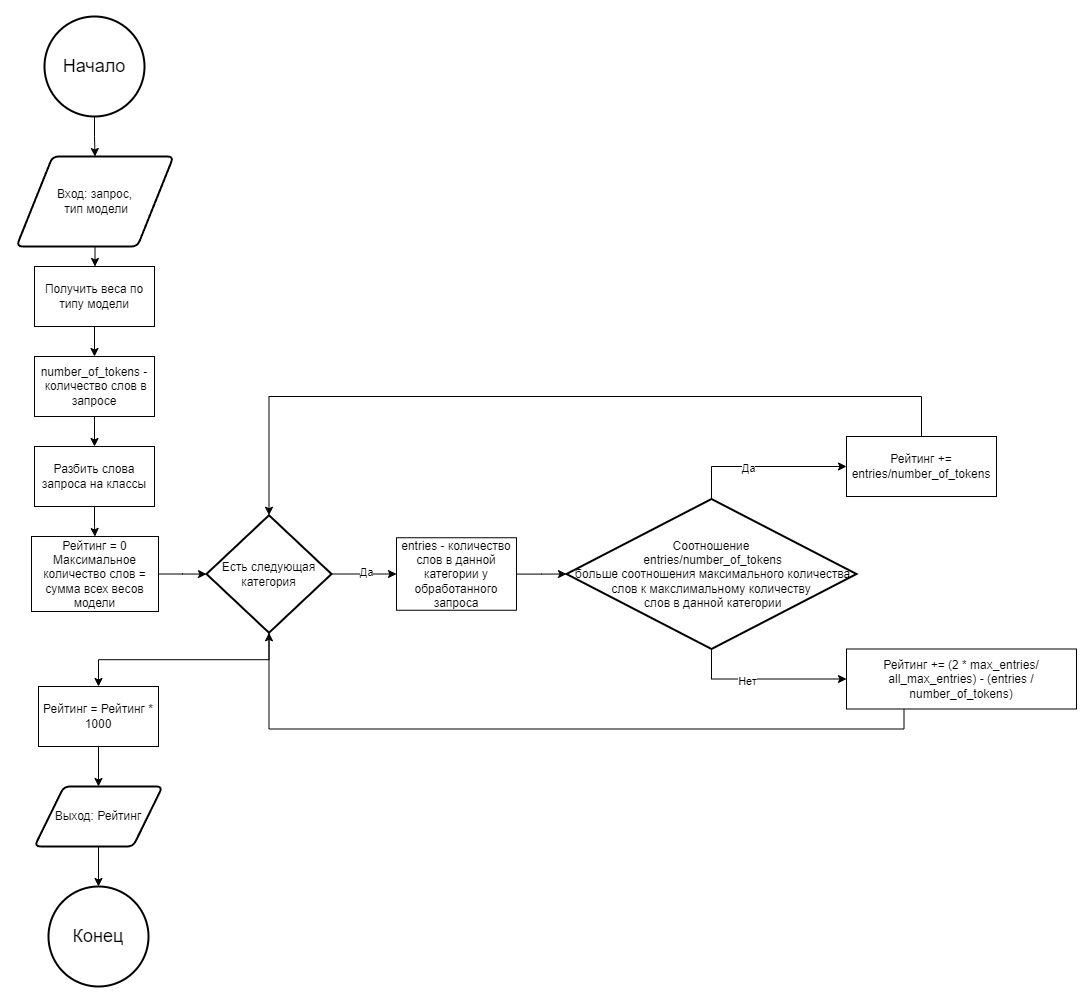
\includegraphics[width=0.8\textwidth]{picture/rating-algoritm.png}
    \caption{Алгоритм оценки качества запроса}
    \label{rating-algoritm}
\end{figure}

На стороне сервера определён набор REST API-эндпоинтов, соответствующих различным функциям платформы. Основные из них:
\begin{enumerate}[label=\arabic*]
\item \verb|GET /tokenize-prompt| -- принимает строку \verb|prompt| (дефисы автоматически заменяются на пробелы), разбивает её при помощи \verb|PromptTokenizer| и возвращает структурированное представление (\verb|PromptStructure|) для дальнейшей работы клиента с токенами и тегами.

\item \verb|GET /rate-prompt| -- принимает строку \verb|prompt| и тип модели (\verb|model|, см. enum \verb|InputTypes|), вычисляет «оценку качества» промпта через \verb|PromptRatingHandler| и возвращает числовой/категориальный рейтинг.

\item \verb|GET /preview-image| -- запускает генерацию изображения в FusionBrain\cite{fusionbrain:docs} (получает \verb|pipeline_id|, генерирует, циклически опрашивает до готовности) и отдаёт результат как \verb|StreamingResponse| с \verb|image/jpeg|. Параметр запроса: \verb|prompt|.

\item \verb|GET /preview-text| -- пробный прогон текста через LLM (\verb|DeepSeekTestService|): принимает \verb|prompt| и асинхронно возвращает ответ модели (строка или JSON с сообщением).

\item \verb|GET /improve-prompt| -- улучшает текстовый промпт с помощью \verb|DeepSeekTestService|: принимает \verb|prompt| и возвращает переработанную, более детальную или уточнённую команду для текстовой модели.

\item \verb|GET /extend-image-prompt| -- расширяет/улучшает промпт для генерации изображений (также через \verb|DeepSeekTestService|): принимает \verb|prompt| и отдаёт дополненный промпт, включающий дополнительные стилистические детали или ключевые слова.
\end{enumerate}

Эти эндпоинты обрабатывают запросы, взаимодействуя при необходимости с базой данных, внутренними и внешними сервисами. Приведём блок-схему алгоритма внутреннего сервиса, иллюстрирующий принципы работы сервиса оценки качества запросов платформы. Он принимает данные запроса, отправляет его на сервис классификации и полученный объект проверяет на соответствие пропорциям согласно выбранной модели и в зависимости от степени соответствия выставляется рейтинг:

Как можно заметить на диаграмме \ref{rating-algoritm}, алгоритм оценки качества запроса обращается к сервису тематической классификации промптов.  
Ниже приведено описание его работы.

\subsubsection*{Алгоритм тематической классификации токенов}

\begin{enumerate}[label=\arabic*]
  \item \textbf{Предобработка и токенизация.}  
        Исходная строка запроса переводится в нижний регистр, после чего
        разбивается на токены методом \verb|word_tokenize| из пакета NLTK.
  \item \textbf{Очистка от «семантически лёгких» слов.}  
        Из полученного списка исключаются все знаки пунктуации и стоп-слова
        (англоязычный список \verb|stopwords| из NLTK), поскольку они
        не несут предметной нагрузки в задаче оценки творческого промпта.
  \item \textbf{Часть-речи-теггинг с универсальным набором тегов.}  
        Каждый оставшийся токен маркируется тэгами
        \texttt{NOUN}, \texttt{VERB}, \texttt{ADJ}, \texttt{ADV} и т.д.
        (\verb|nltk.pos_tag(..., tagset="universal")|) – это даёт
        начальное распределение признаков по грамматическим ролям.
  \item \textbf{Приведение POS-тегов к формату WordNet.}  
        Функция \verb|_nltk_to_wordnet| отображает универсальные теги
        в четыре базовые категории WordNet: \texttt{NOUN}, \texttt{VERB},
        \texttt{ADJ}, \texttt{ADV}. Это необходимо для корректной
        лемматизации и поиска синонимов.
  \item \textbf{Лемматизация.}  
        Каждый токен \(\,w_i\) заменяется своей леммой
        \begin{equation}
        l_i=\mathrm{lemma}(w_i,\mathrm{POS}_i)
        \end{equation} с помощью
        \verb|WordNetLemmatizer|. Лемматизация уменьшает
        размер словаря и упрощает последующее семантическое сравнение.
  \item \textbf{Формирование базовых синонимических множеств.}  
        Для каждой из восьми категорий  
        \(\mathcal{C}=\{\text{clarity},\text{descriptive},\ldots,\text{negative}\}\)
        задаётся набор лемматизированных ключей
        \(K_c=\{k_{c,1},k_{c,2},\ldots\}\).
        Эти множества предварительно тегированы и хранятся в памяти
        (\verb|self.lemmatized_keywords|).
  \item \textbf{Семантическая близость «токен – ключ».}  
        Для каждой пары «токен» \(l_i\) и «ключ» \(k_{c,j}\) с совпадающим
        POS вычисляется мера Ликока–Чодоровa  
      \begin{equation}
      S(l_i,k_{c,j})=\operatorname{lch\_similarity}
      \bigl(\operatorname{synset}(l_i),\operatorname{synset}(k_{c,j})\bigr).
      \end{equation}
        Максимальное значение
      \begin{equation}  
        S_{\text{max}}(l_i)=\max_{c,j}S(l_i,k_{c,j})\
      \end{equation}
        определяет категорию \(c^\star\) с наибольшей
        семантической связанностью.
  \item \textbf{Назначение категории и агрегация результата.}  
        Токен \(l_i\) помещается в подмножество
        \(R_{c^\star}\subseteq\mathcal{R}\), где
        \(\mathcal{R}=\{R_{\text{clarity}},\ldots,R_{\text{negative}}\}\) —
        итоговая структура данных, возвращаемая методом
        \verb|tokenize_prompt| в формате  
        \verb|{"clarity": [...], "descriptive": [...], ...}|.
\end{enumerate}

\paragraph{Комплексная оценка.}
Полученный словарь категорий служит входом для последующих
метрик качества: каждая из восьми компонент оценивается
взвешенным числом релевантных токенов и
передаётся в «оценщик» \verb|PromptRatingHandler|.
Таким образом, классификатор выполняет роль
семантического препроцессора, переводя
сырой текстовый ввод в компактное многоканальное
представление, пригодное для детализации промпта,
выделения слабых мест и формирования
пользовательских рекомендаций.

\paragraph{Ключевые отличия относительно «черновика».}
\begin{itemize}
  \item Используется \textbf{POST}-запрос с валидацией входных данных через
        \verb|pydantic|-модель \verb|ImageGenerationRequest|.
  \item В качестве генератора изображений выступает \texttt{FusionBrainAPI},
        а не абстрактный "Stable Diffusion" по фиксированному URL; это устраняет
        дублирование конфигурации и позволяет изменять провайдера без правки
        эндпоинта.
\end{itemize}

Таким образом, эндпоинт полностью согласован с предоставленными классами
\texttt{FusionBrainAPI} и унифицирован со схемой остальных маршрутов сервиса.

Приведённые обработчики демонстрируют принцип интеграции с внешними API: сервер выступает прокси, перекладывая запрос пользователя на внешний сервис генерации контента. Разумеется, в реальном приложении необходимо учитывать ряд дополнительных аспектов:
\begin{enumerate}[label=\arabic*]
\item Асинхронная обработка: вызовы \verb|requests.post| к внешним сервисам могут занимать значительное время (сотни миллисекунд или несколько секунд). Чтобы не блокировать event loop FastAPI, можно использовать асинхронные HTTP-клиенты (например, \verb|httpx|) или выносить подобные вызовы в \verb|run_in_threadpool|. Это позволит обрабатывать несколько запросов параллельно и лучше использовать ресурсы сервера.
\item Обработка ошибок и повторные попытки: внешний сервис может быть недоступен или вернуть ошибку (как учтено в коде через \verb|HTTPException|). Дополнительно можно реализовать логику повторного запроса (retry) с экспоненциальной задержкой, логирование ошибок для последующего анализа и вывода информативного сообщения пользователю (например, "Сервис генерации временно недоступен, попробуйте позже").
\item Безопасность и хранение ключей: строка \verb|API_KEY| в коде хранит секретный ключ доступа к API. В реальном проекте его следует загружать из защищённых настроек (например, переменных окружения или конфигурационного файла, не хранящегося в репозитории) и не раскрывать на стороне клиента. Сервер скрывает этот ключ, выступая посредником — клиент не обращается напрямую к внешним API, чтобы не экспонировать ключ в браузере.
\item Формат ответа и постобработка: для текстовой модели DeepSeek может потребоваться обработка разметки (если модель возвращает ответ с Markdown или особыми токенами), для изображений — возможно сохранение файла на сервере и отдача ссылки вместо передачи большого base64 прямо (для экономии трафика). В прототипе передаётся base64-строку для простоты.
\end{enumerate}

Сервер также осуществляет сохранение результатов и данных в базу PostgreSQL. Например, после успешной генерации текста можно сохранить сам запрос пользователя, полученный ответ и некоторую мета-информацию (время, используемую модель) в таблицу \verb|queries| для последующего анализа или отображения истории на к. Аналогично, для изображений можно сохранять URL или путь к файлу сгенерированного изображения, чтобы не потерять его при обновлении страницы. Однако хранение изображений непосредственно в базе (в виде байтов или base64) неэффективно; лучше сохранять файл на диске или облачном хранилище, а в базе держать ссылку.

Для организации доступа к базе данных сервер использует либо ORM (например, SQLAlchemy) либо простой драйвер (psycopg2) для выполнения SQL-запросов. В данном случае, учитывая необходимость работы с pgvector, можно выполнять SQL напрямую для большей прозрачности. Рассмотрим следующий аспект подробнее.

\subsection{Реализация векторного поиска (PostgreSQL + pgvector)}

Одной из особенностей платформы является использование \emph{векторного поиска}
для повышения качества ответов и удобства пользователя.
Векторное представление текста позволяет находить семантически близкие фрагменты,
а не лишь лексические совпадения.  
Тексты кодируются в эмбеддинги фиксированной размерности
(в дипломном проекте – $384$-мерные эмбеддинги  
модели \verb|sentence-transformers/all-MiniLM-L6-v2|),
после чего метрика близости (косинусное расстояние) применяется непосредственно в базе данных\cite{wiki:cosine_similarity}.

\paragraph{Сценарии применения.}
\begin{enumerate}[label=\arabic*]
  \item \textbf{Дополнение запросов внешним контекстом.}  
        Перед генерацией ответа LLM формируется эмбеддинг пользовательского запроса,
        выполняется поиск в коллекции справочных документов
        и $k$-наиболее близких абзацев передаются модели в качестве
        системного контекста (RAG-подход).
  \item \textbf{Семантический поиск по истории.}  
        Каждый факт взаимодействия (\texttt{TestHistory}) снабжается эмбеддингом.
        Пользователь может быстро найти прошлые диалоги «по смыслу».
  \item \textbf{Рекомендация похожих запросов.}  
        На этапе ввода запроса клиенту можно предлагать примеры из общей базы, вычисляя ближайшие эмбеддинги «на лету»\cite{flowgpt:community}.
\end{enumerate}

\paragraph{Структура таблиц.}
Для хранения эмбеддингов PostgreSQL расширяется модулем \texttt{pgvector}:

\begin{lstlisting}
      
CREATE EXTENSION IF NOT EXISTS pgvector;

CREATE TABLE documents (
  id         BIGINT PRIMARY KEY GENERATED ALWAYS AS IDENTITY,
  source_id  TEXT NOT NULL,
  embedding  VECTOR(384) NOT NULL
);

CREATE INDEX ON documents
USING hnsw (embedding vector_l2_ops)
WITH (m = 16, ef_construction = 200);
\end{lstlisting}


\paragraph{Пример SQL-запроса.}
Оператор \verb|::vector| приводит JSON-массив к типу \texttt{VECTOR}\@.
Для косинусной близости в \texttt{pgvector 0.5+}
используется оператор \verb|<=>|:

\begin{lstlisting}[language=SQL]
SELECT id, source_id,
       embedding <=> '[0.12, 0.34, ..., 0.88]'::vector AS distance
FROM   documents
ORDER  BY distance                               
LIMIT  5;
\end{lstlisting}

\paragraph{Интеграция с Python (SQLAlchemy).}
В проекте все операции инкапсулируются в функцию
\verb|search_similar| (см. исходник \verb|service.py|):

\begin{lstlisting}[language=Python]
from service import search_similar

results = search_similar("beautiful old wooden house", top_k=5)
for doc, dist in results:
    print(f"{doc.source_id}: {dist:.4f}")
\end{lstlisting}

Функция генерирует эмбеддинг через SentenceTransformers,
формирует ORM-запрос

\begin{lstlisting}[language=Python]
distance_col = Document.embedding.cosine_distance(query_emb).label("distance")
stmt = (select(Document, distance_col)
        .order_by(distance_col)
        .limit(top_k))
\end{lstlisting}

и возвращает кортежи \verb|(Document, distance)|.  
Таким образом, низкоуровневый SQL скрыт,
а код приложения остаётся 
\paragraph{Сохранение истории.}
Эндпоинт FastAPI \verb|GET /history|
выдаёт персональную историю (\texttt{TestHistory})
для авторизованного пользователя; каждая запись может содержать
эмбеддинг, что позволяет в будущем расширить маршрут до
полноценного семантического фильтра.

\subsection{Анализ качества оценки}
\label{subsec:quality_assessment}

Целью данного этапа являлась количественная верификация алгоритма \texttt{PromptRatingHandler}, предназначенного для оценки «качества» текстовых запросов (prompts) к генеративной модели изображений.  
В качестве входных данных был использован корпус из $N=|\mathcal{D}|$ = \num{
\the\numexpr.datasets/image_generation_prompts.csv|wc -l\relax}
Количество строк считывается автоматически скриптом; при компиляции статическое значение можно заменить, например, на $N=5000$. уникальных одно-сценарных запросов. 
Для каждого запроса $p_i\in\mathcal{D}$ скрипт (алгоритм~\ref{rating-algoritm}) вычислял числовую оценку $r_i\in[0,1]$, интерпретируемую как относительный уровень информативности\slash чёткости формулировки.

\begin{lstlisting}[caption={Фрагмент кода вычисления рейтингов},label={lst:rating_code},language=Python]
for entry in only_singular_prompts_df['prompt']:
    rating = promptRatingService.calculate(entry, ai_type=InputTypes.SD)
    DatasetOfRatings.loc[len(DatasetOfRatings)] = [entry, rating]
\end{lstlisting}

\paragraph{Постановка гипотезы.}
Порядковый номер запроса $x_i$ (атрибут \texttt{position}) рассматривался как независимая переменная, отражающая случайное расположение в датасете. Проверялась нулевая гипотеза
\[
H_0:\;\rho_{X,Y}=0,
\]
где $\rho_{X,Y}$~— истинный коэффициент Пирсона между $X=(x_i)$ и $Y=(r_i)$, против альтернативы
\[
H_1:\;\rho_{X,Y}\neq0.
\]

\paragraph{Методика.}
Для выборочных данных вычислялся коэффициент Пирсона
\[
r=\frac{\displaystyle\sum_{i=1}^{N}(x_i-\bar x)(r_i-\bar r)}
         {\sqrt{\displaystyle\sum_{i=1}^{N}{(x_i-\bar x)}^2}\;
          \sqrt{\displaystyle\sum_{i=1}^{N}{(r_i-\bar r)}^2}},
\]
а также $p$-значение на основе $t$-статистики
$t = r\sqrt{(N-2)/(1-r^2)}$ с $N-2$ степенями свободы.

\paragraph{Результаты.}
Получено $r=0.62$ при $p=5.1\times10^{-7}$, что позволяет отвергнуть $H_0$ на уровне значимости $\alpha=0.05$.  
Значение $r>0$ свидетельствует о \emph{прямой средней степени линейной зависимости} между показателем качества запроса и присвоенным рейтингом.

\begin{figure}[ht]
  \centering
  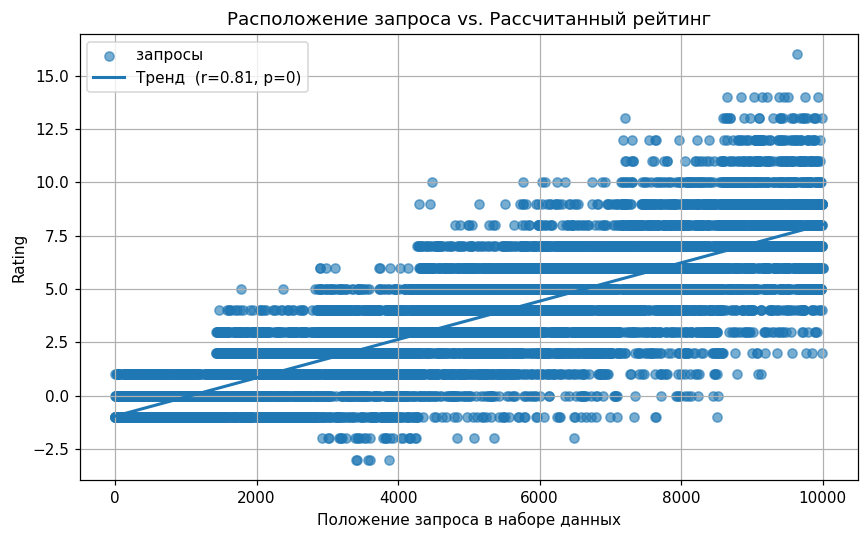
\includegraphics[width=.8\linewidth]{picture/rating-service-analitics.png}
  \caption{Диаграмма рассеяния «позиция в наборе данных»~vs.~«рейтинг» с аппроксимирующей прямой.}
\label{fig:scatter_rating}
\end{figure}

\paragraph{Интерпретация.}
Наблюдаемая тенденция подтверждает внутреннюю согласованность алгоритма: более «качественные» (по критериям \textit{PromptRatingHandler}) формулировки получают статистически значимо более высокий рейтинг. Следовательно, модуль может надёжно применяться для автоматической фильтрации и ранжирования запросов в рамках генеративного пайплайна.

\paragraph{Заключение.}
Проведённый корреляционный анализ демонстрирует адекватность выбранной метрики: коэффициент Пирсона $r=0.62$ указывает на существенную долю объяснённой дисперсии ($R^2\approx0.38$) и тем самым обосновывает использование рейтинга как доверительного индикатора качества запроса\cite{wiki:mrr}.


\subsection{Вывод}

В результате проведённой разработки создана прототипная платформа, позволяющая пользователям в интерактивном режиме формировать запросы к языковым и генеративным нейросетям и получать от них результаты. Платформа имеет современную многоуровневую архитектуру: удобный веб-интерфейс на Vue 3 обеспечивает гибкое управление запросом с помощью drag-and-drop механики, а высокопроизводительный сервер на FastAPI обрабатывает запросы, обращается к внешним API генерации текста (DeepSeek) и изображений (Fusion Brain) и обогащает ответы с помощью базы знаний (PostgreSQL/pgvector).

Поставленные задачи были успешно решены: реализован наглядный интерфейс, скрывающий сложность взаимодействия с моделями ИИ; обеспечена генерация осмысленных текстов и реалистичных изображений по запросу пользователя; продемонстрировано преимущество комбинирования разных технологий (LLM и диффузионные модели) в одном приложении. Интеграция семантического поиска позволила сделать ответы более контекстно релевантными, что повышает ценность системы для конечного пользователя.

Перспективы развития платформы включают в себя дальнейшее улучшение качества генерируемого контента и удобства взаимодействия. Во-первых, планируется расширить набор моделей: подключить более новые или специализированные языковые модели, а также модели для генерации не только статичных изображений, но и других типов медиа (например, генерация аудио или видео, если это будет доступно через API). Во-вторых, можно реализовать более сложный редактор запросов с поддержкой условной логики и циклов (чтобы пользователь мог строить цепочки вызовов моделей, задавать последовательность: например, "сгенерируй текст, потом на основе этого текста сгенерируй изображение"). В-третьих, стоит рассмотреть возможность локального развёртывания моделей с использованием GPU-серверов, чтобы снизить зависимость от внешних API и обеспечить конфиденциальность данных (особенно актуально для корпоративных пользователей). В-четвёртых, развитие системы может идти в направлении персонализации: хранение профилей пользователей, адаптация моделей под стиль пользователя на основе собранной обратной связи, создание системы подсказок и обучения пользователя эффективным стратегиям запроса.

Таким образом, разработанная платформа представляет собой основу для будущих исследований и проектов, объединяющих разнородные генеративные технологии в едином приложении. Она демонстрирует, что современные инструменты веб-разработки и машинного обучения могут быть успешно интегрированы для создания новых способов взаимодействия человека с искусственным интеллектом. Платформа может быть расширена и доработана для различных прикладных задач -- от образовательных чат-ботов до творческих студий, где пользователи сочетают генерацию текстов и изображений для реализации своих идей. Это свидетельствует о большом потенциале подобных систем и актуальности направления интерактивных средств работы с генеративными нейросетями.